\documentclass[12pt]{article}
\usepackage{xltxtra}
\usepackage{xgreek}
\usepackage[a4paper, inner=2.5cm, outer=2.5cm, top=3cm, bottom=3cm, bindingoffset=0.5cm]{geometry}
\setmainfont[Mapping=tex-text]{GFS Artemisia}
\usepackage{amsfonts}
\usepackage{multicol}
\usepackage{url}
\usepackage{hyperref}
\usepackage[dvipsnames]{xcolor}
\linespread{1.25}

\usepackage[acronym]{glossaries}

\providecommand{\keywords}[1]
{
  \small	
  \textbf{\textit{Λέξεις κλειδιά:}} #1
}

\makeglossaries


\newglossaryentry{opengl}
{
    name=OpenGl,
    description={Open Graphics language}
}


\newglossaryentry{filter}
{
    name=ηθμός,
    description={Πίνακας φίλτρο}
}

\newglossaryentry{convolution}
{
    name=συνέλιξη,
    description={Μαθηματική πράξη μεταξύ δύο συναρτήσεων}
}

\newglossaryentry{RGB}
{
    name=RGB,
    description={Χρωματικός χώρος (Κόκκινο, Πράσινο, Μπλε)}
}

\newglossaryentry{glsl}
{
    name=glsl,
    description={OpenGL Shading Language}
}

\setlength{\parskip}{1mm}

\begin{document}

%\maketitle
% To add this template to the main.tex file, just add the command "\include{titlePageSLU} after "\begin{docuemnt}" in the main.tex file


% In this segment, enter the desired data to be shown at the title page
\newcommand{\thesisAuthora}{Στεφανάτου Νεφέλη (snefeli@uth.gr)}
\newcommand{\thesisAuthorb}{Λάζαρο Κων/νο-Παναγιώτη (lakonstant@uth.gr)}

\newcommand{\thesisTitle}{ΔΙΔΙΑΣΤΑΤΗ ΣΚΗΝΗ }
\newcommand{\thesisSubTitle}{ΕΡΓΑΣΙΑ ΓΙΑ ΤΟ ΜΑΘΗΜΑ ΓΡΑΦΙΚΗ ΥΠΟΛΟΓΙΣΤΩΝ }
\newcommand{\professor}{Δρακόπουλος Βασίλειος}
\newcommand{\academicYear}{2020-2021}

%------------------------------------------------------------------------------
\begin{titlepage}
\thispagestyle{empty}
%\myfont

% Use this line of code if both SLU loggo and company/other institution loggo is desired. The positions are possible to change with the \hspace and \vspace syntax.

\begin{figure}
\centering
\vspace{-2cm}
    \hspace*{0cm}
\includegraphics[width = 0.2\textwidth]{uth_logo.png}\hspace*{0cm}
\end{figure}


\definecolor{uthred}{RGB}{122, 8, 44}
\centering 
\textcolor{uthred} {\large \textbf{ΠΑΝΕΠΙΣΤΗΜΙΟ ΘΕΣΣΑΛΙΑΣ}}\\
\vspace{0.2cm}
\textcolor{uthred}{\textbf{ΤΜΗΜΑ ΠΛΗΡΟΦΟΡΙΚΗΣ ΜΕ ΕΦΑΡΜΟΓΕΣ ΣΤΗ ΒΙΟΪΑΤΡΙΚΗ}}\\

\rule[-0.2cm]{\linewidth}{0.5pt}

\vspace{3cm}
\par
\noindent
\Huge
\centering
\textbf{\thesisTitle}\\
\vspace{0.2cm}
\small
\par
\noindent
\thesisSubTitle\\
%\rule[0.3cm]{\linewidth}{2pt}
\Large


\vspace{2cm}
\noindent
\Large
ΕΚΠΟΝΗΘΗΚΕ ΑΠΟ ΤΟΥΣ:\\
\textbf{\thesisAuthora}\\
\textbf{\thesisAuthorb}\\
\vspace{3 cm}

\par \noindent
\Large
ΔΙΔΑΣΚΩΝ ΚΑΘΗΓΗΤΗΣ:\\ \textbf{\professor}\\
\vspace{2.5cm}

\rule[0.2cm]{\linewidth}{0.5pt}

ΑΚΑΔΗΜΑΪΚΟ ΕΤΟΣ: \academicYear

\end{titlepage}

\tableofcontents
\clearpage
\begin{abstract}
Η εργασία αυτή αναφέρεται στην υλοποίηση μιας διδιάστατης σκηνής με κώδικα καθώς και στην σύγκριση των αποτελεσμάτων διαφορετικών συνελίξεων πάνω σε αυτήν. Ό κώδικας αναπτύχθηκε σε γλώσσα C με χρήση συναρτήσεων της βιβλιοθήκης γραφικών \Gls{opengl}. 

Το πρώτο κεφάλαιο αποτελεί μια συνοπτική ανάλυση του πηγαίου κώδικα που υλοποιήθηκε για τον σχεδιασμό της διδιάστατης σκηνής. 

Στο δεύτερο κεφάλαιο περιγράφεται η υλοποίηση των συνελίξεων της σκηνής, αρχικά με έναν ηθμό συνέλιξης 3x3 και στην συνέχεια με έναν ηθμό 3x3 που έχει όλα τα βάρη του ίσα. 

Έπειτα ακολουθεί η σύγκριση των διαφορετικών αποτελεσμάτων των δύο συνελίξεων. 

Τέλος γίνεται διεξαγωγή συμπερασμάτων και καταγράφονται οι πηγές που χρησιμοποιήθηκαν για την εκπόνηση της εργασίας. 


\begin{center}
 \large Abstract
\end{center}

This paper presents the implementation of a simple two dimensional scene. It also includes a comparison of the results that occur by applying two different convolution filters to the scene. The code was developed in C using functions from the OpenGl graphics library. 

The first chapter is a brief analysis of the source code implemented for drawing the two-dimensional scene.

The second chapter describes the implementation of the two convolutions. The first one is implemented using a 3x3 convolution filter and the second one is implemented using a 3x3 filter with equal weights. 

Then follows the comparison of the different results of the two convolutions. 

Finally, conclusions are drawn and the sources used to implement the work are recorded.
\end{abstract}

\keywords{μεταδιήθηση \cite{CompGraphicsOpenGL}, ηθμός, συνέλιξη \cite{GraphicsReality}, glsl \cite{learnopengl}, glfw \cite{glfw}}

\section{Εισαγωγή}
Με τον όρο διδιάστατα γραφικά εννοούμε την δημιουργία ψηφιακών εικόνων από διδιάστατα μοντέλα σε υπολογιστή. Σκοπός αυτής της εργασίας είναι η περιγραφή της χάραξης μιας απλής διδιάστατης σκηνής η οποία αποτελείται από ένα σύνολο τριγώνων. Με βάση τα ζητούμενα, η σκηνή θα χαραχθεί σε τριπλάσια ευκρίνεια και στη συνέχεια θα υποστεί επεξεργασία με χρήση δύο ηθμών. Ο πρώτος είναι ο ηθμός συνέλιξης 3x3 και ο δεύτερος είναι ένας ηθμός 3x3 ο οποίος έχει όλα του τα βάρη ίσα. Τα βάρη αμφότερων ηθμών είναι κανονικοποιημένα. Ακολουθεί αναλυτική περιγραφή της διαδικασίας καθώς και σύγκριση των διαφορετικών αποτελεσμάτων.

\section{Χάραξη διδιάστατης σκηνής}
Αρχικά, συμπεριλαμβάνονται (με include) οι βιβλιοθήκες που είναι απαραίτητες για την χάραξη της διδιάστατης σκηνής. Στην συνέχεια αρχικοποιούμε τις συντεταγμένες και τα χρώματα που θα έχουν οι κορυφές των τριγώνων της σκηνής. Η κάθε κορυφή περιγράφεται από 2 διανύσματα. Το ένα είναι το διάνυσμα θέσης (x,y) και το άλλο είναι το διάνυσμα χρώματος \gls{RGB}.

Με την συνάρτηση error\_callback γίνεται έλεγχος για πιθανά λάθη κατά τη διάρκεια εκτέλεσης του προγράμματος. Σε περίπτωση που υπάρξει κάποιο σφάλμα, θα τυπωθεί στην οθόνη αντίστοιχο μήνυμα. Με την συνάρτηση key\_callback γίνεται έλεγχος για το αν ο χρήστης έχει πατήσει κάποιο πλήκτρο (αν ο χρήστης πατήσει το πλήκτρο escape τότε θα κλείσει το παράθυρο της σκηνής). Η εργασία αναπτύχθηκε σε λειτουργικό σύστημα linux.

Στην κύρια συνάρτηση του προγράμματος (main) αρχικοποιείται η βιβλιοθήκη glfw (ελαφριά βοηθητική βιβλιοθήκη για χρήση με OpenGl) και δημιουργείται ένα παράθυρο λειτουργίας με ορίσματα το πλάτος και το ύψος της επιφάνειας σχεδίασης της εφαρμογής σε pixels, στο οποίο θα εμφανιστεί η διδιάστατη σκηνή. 

Στην διδιάστατη σκηνή απεικονίζεται ένα ρομπότ το οποίο είναι σχεδιασμένο με βάση την τεχνοτροπία του κινέζικου παιχνιδιού tangram. Χρησιμοποιώντας την εντολή glfwSwapInterval σχεδιάζεται πρώτα το τρέχον πλαίσιο (frame) πριν αρχίζει να σχεδιάζεται το επόμενο. Οι σκιαστές (shaders) συνδέουν τον κώδικα με τα γραφικά. Για να χρησιμοποιήσουμε τους shaders, απλά τους καλούμε καθώς είναι γραμμένοι σε μια ειδική γλώσσα που λέγεται \gls{glsl} και βρίσκονται πάνω από την κύρια συνάρτηση (πηγαίο αρχείο main.c, γραμμές 114-171). Υπάρχουν δύο τύποι shader: 

\begin{enumerate}
  \item O vertex shader. Μετατρέπει τις συντεταγμένες των κορυφών κάθε αρχεγόνου / σχήματος (στην περίπτωσή μας τρίγωνα) , σε συντεταγμένες σχεδίασης.
  \item O fragment shader. Υπολογίζει το χρώμα και άλλα χαρακτηριστικά κάθε "θραύσματος" της σκηνής.
\end{enumerate}

 Με τον όρο θραύσμα εννοούμε την μονάδα απόδοσης που επηρεάζει το πολύ ένα μεμονωμένο εικονοστοιχείο (pixel) εξόδου. Το πρόσωπο του ρομπότ είναι τετράγωνο. Για να φτιαχτεί, ενώνονται τρία τρίγωνα μεταξύ τους με κατάλληλο τρόπο.
 
 Με την εντολή glViewport ορίζεται η θύρα θέασης μέσα στο παράθυρο λειτουργίας. Εκεί θα σχεδιαστεί τελικά η διδιάστατη σκηνή. 

Χρησιμοποιείται η εντολή glClear(GL\_COLOR\_BUFFER\_BIT) έτσι ώστε να καθαριστεί ο ρυθμιστής (buffer) χρώματος. 

Με την εντολή glfwSwapBuffers(window) γίνεται εναλλαγή των ρυθμιστών πλαισίου (πρόσθιο και οπίσθιο frame buffer). 

Με την εντολή glDrawArrays(GL\_TRIANGLES, 0, 60) χαράζονται τα τρίγωνα έτσι ώστε να παραχθεί η τελική διδιάστατη σκηνή. Το όρισμα 60 δείχνει πόσες συνολικά είναι οι κορυφές της σκηνής (σχήμα~\ref{fig:robotOriginal}).

\begin{figure}[!h]
\centering
    {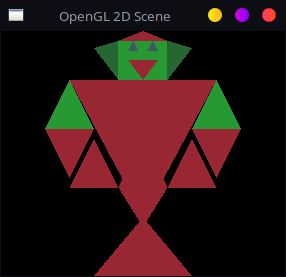
\includegraphics[width=0.5\textwidth]
    {robot_original.png}}
    \caption{\label{fig:robotOriginal} Απλή διδιάστατη σκηνή}
\end{figure}
%\clearpage

\section{Χάραξη διδιάστατης σκηνής σε τριπλάσια ευκρίνεια}
Θα πρέπει να χαραχθεί η ίδια διδιάστατη σκηνή σε τριπλάσια ευκρίνεια (s = 3). Αυτό γίνεται πολύ εύκολα, απλά αντικαθιστώντας τις τιμές του μήκους και του πλάτους του παραθύρου με τις τριπλάσιες. Μπορούμε είτε να αλλάξουμε τις τίμες στις τριπλάσιες κατά της αρχικοποίηση των μεταβλητών αυτών. Εναλλακτικά μπορούμε να πολλαπλασιάσουμε τις ήδη υπάρχουσες τιμές ύψους και πλάτους με το τρία (σχήμα~\ref{fig:robotTriple}).

\begin{figure}[!h]
\centering
    {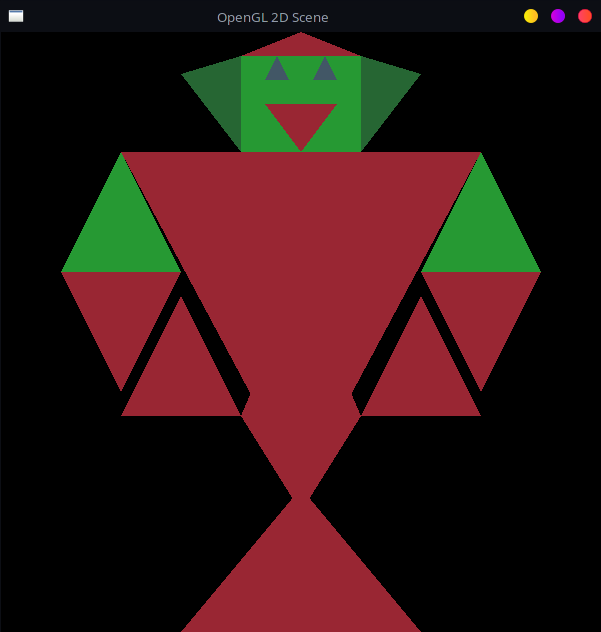
\includegraphics[width=1\textwidth]
    {robot_triple_size.png}}
    \caption{\label{fig:robotTriple} Διδιάστατη σκηνή σε τριπλάσια ευκρίνεια}
\end{figure}
\clearpage



\section{Μεταδιήθηση με γκαουσιανό ηθμό συνέλιξης}
Κατά τη διαδικασία της συνέλιξης ο \gls{filter} διατρέχει την εικόνα και κάθε φορά υπολογίζεται το άθροισμα των γινομένων των στοιχείων του ηθμού με τα αντίστοιχα εικονοστοιχεία (pixels) της εικόνας. Στην εικόνα εξόδου το αποτέλεσμα της συνέλιξης αποδίδεται στο κεντρικό pixel του παραθύρου. Για να επιτευχθεί αυτή η διαδικασία πρέπει απλά να τοποθετήσουμε σε σχόλιο την γραμμή 166 (οπού καλείται ο fragment shader με τα κανονικά χρώματα της σκηνής), και να ενεργοποιηθεί η γραμμή 167 όπου καλείται το αποτέλεσμα της διαδικασίας της συνέλιξης με τον γκαουσιανό ηθμό 3x3(σχήμα~\ref{fig:robotGauss}).


\begin{figure}[!h]
\centering
    {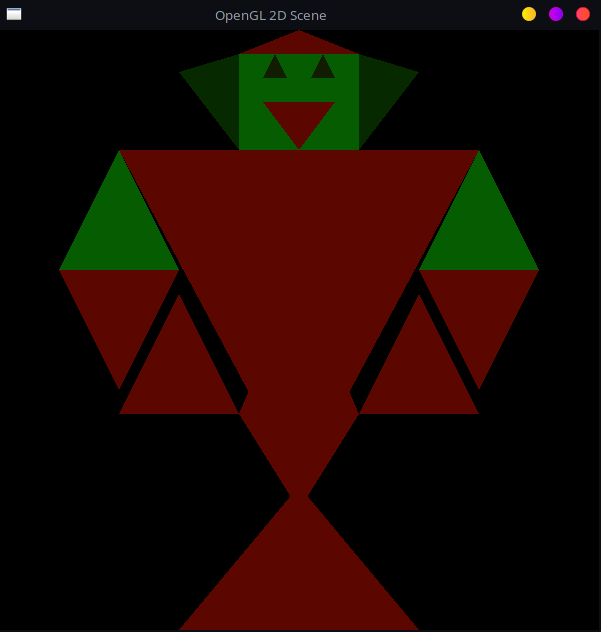
\includegraphics[width=1\textwidth]
    {robot_gaussian_conv.png}}
    \caption{\label{fig:robotGauss} Αποτέλεσμα μεταδιήθησης με γκαουσιανό ηθμό συνέλιξης}
\end{figure}
\clearpage

\section{Μεταδιήθηση με ηθμό με όλα τα βάρη ίσα}
Προκειμένου να εκτελεστεί η \gls{convolution} της εικόνας με τον ηθμό ο οποίος έχει όλα τα βάρη του ίσα το μόνο που χρειάζεται να γίνει είναι να τοποθετηθεί σε σχόλιο η γραμμή 167 και να ενεργοποιηθεί η γραμμή 168 όπου καλείται το αποτέλεσμα της συνέλιξης με τον 3x3 ηθμό με όλα τα βάρη ίσα (σχήμα~\ref{fig:robotUniform}).

\begin{figure}[!h]
\centering
    {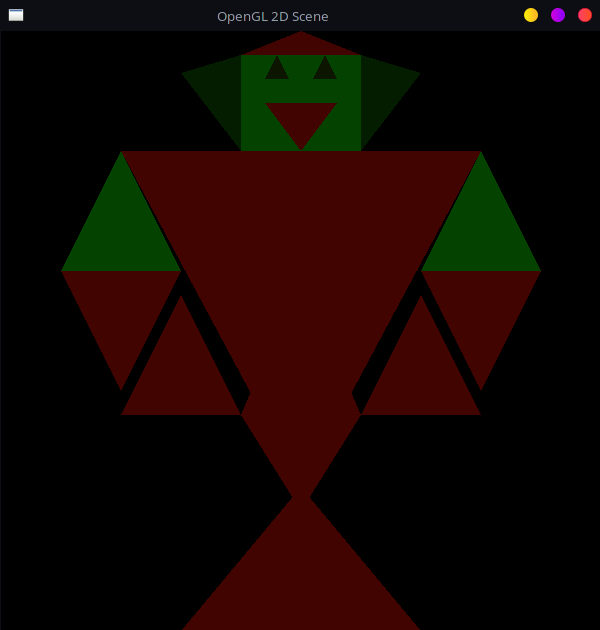
\includegraphics[width=1\textwidth]
    {robot_uniform_conv.png}}
    \caption{\label{fig:robotUniform} Αποτέλεσμα μεταδιήθησης με ηθμό με όλα τα βάρη ίσα}
\end{figure}
\clearpage

\section{Συμπεράσματα}
Αρχικά η χάραξη της διδιάστατης σκηνής γίνεται σε παράθυρο διαστάσεων 200x200. Ακολούθως οι διαστάσεις του παραθύρου της σκηνής και κατ’ επέκταση η ευκρίνειά της αυξάνονται καθώς πολλαπλασιάζονται το πλάτος και το ύψος του παραθύρου με το 3. Η συνέλιξη της σκηνής με τον γκαουσιανό ηθμό οδήγησε σε μεταβολές των χρωμάτων της εικόνας. Υπάρχει επίσης μείωση στην ένταση της φωτεινότητας. Η συνέλιξη της σκηνής με τον ηθμό που έχει όλα τα βάρη ίσα, έχει ως αποτέλεσμα παρόμοιες χρωματικές αλλαγές με αυτές τις πρώτης συνέλιξης. Το περιεχόμενο της εικόνας είναι όμως λιγότερο διακριτό καθώς έχει μειωθεί η ένταση της φωτεινότητας ακόμη περισσότερο. Και στις δύο περιπτώσεις συνέλιξης, η σκηνή είναι λιγότερο ξεκάθαρη, τα χρώματα αλλάζουν χωρίς όμως να υπάρχουν μεγάλες διακυμάνσεις.


\section{Επίλογος}
Εν κατακλείδι, η διδιάστατη σκηνή υλοποιήθηκε σε γλώσσα C με χρήση της βοηθητικής βιβλιοθήκης glfw γραφικών OpenGL. Ακολούθησε μια ανάλυση του πηγαίου κώδικα που υλοποιήθηκε για την χάραξη της διδιάστατης σκηνής , σε μια αρχική και στην συνέχεια σε τριπλάσια ευκρίνεια. Έπειτα εκτελέστηκε μεταδιήθηση με γκαουσιανό ηθμό συνέλιξης 3x3, αλλά και με ηθμό συνέλιξης 3x3 ο οποίος είχε όλα τα βάρη ίσα. Με βάση τα κριτήρια της εργασίας αλλά και τα αποτελέσματα κάθε διαδικασίας παρουσιάστηκαν τα τελικά συμπεράσματά μας.



\printglossary

\bibliographystyle{plain}

\bibliography{bibliography}

\end{document}

